\documentclass[12pt]{standalone}
\usepackage{tikz}
\usetikzlibrary{arrows.meta}
\usetikzlibrary{positioning}
\begin{document}
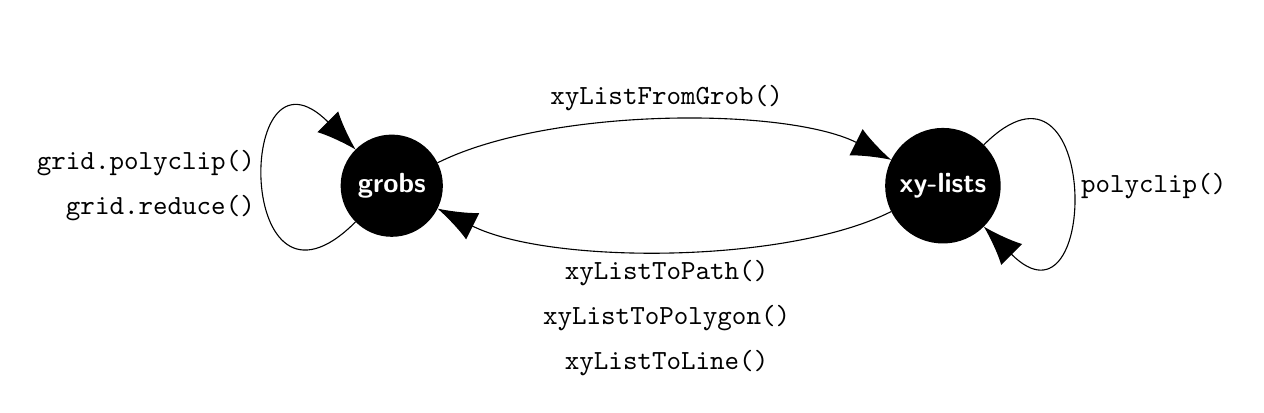
\begin{tikzpicture}  
\path (0, 0) node[circle,minimum size=.5in,fill=black,text=white,draw,thick] (x) {\sffamily{\bfseries{grobs}}};
\path (7, 0) node[circle,minimum size=.5in,fill=black,text=white,draw,thick] (y) {\sffamily{\bfseries{xy-lists}}};
\draw[-{Latex[length=5mm]}] 
       (x) .. controls (-2, -2) and (-2, 2) .. (x) 
          node[pos=.5,anchor=south east]{\ttfamily{grid.polyclip()}}
          node[pos=.5,anchor=north east]{\ttfamily{grid.reduce()}};
\draw[-{Latex[length=5mm]}] 
       (y) .. controls (9, 2) and (9, -2) .. (y) 
          node[pos=.5,anchor=west]{\ttfamily{polyclip()}};
\draw[-{Latex[length=5mm]}] 
       (x) .. controls (2, 1) and (5, 1).. (y) 
          node[pos=.5,anchor=south] (a) {\ttfamily{xyListFromGrob()}};
\draw[-{Latex[length=5mm]}] 
       (y) .. controls (5, -1) and (2, -1) .. (x)
          node[pos=.5,anchor=north] (b) {\ttfamily{xyListToPath()}}
          node[below=0mm of b.south] (c) {\ttfamily{xyListToPolygon()}}
          node[below=0mm of c.south] {\ttfamily{xyListToLine()}};
\end{tikzpicture}
\end{document}
